\section{Methods}
In this section we describe the development methods and the tools which are considered to be used in this project.
A choice is given in both of these areas along with a reasoning for the choices.

\subsection{Development Method}
In this project we are four groups working together.
For this collaboration to work properly it is important that we have a common understanding of the development method we are using.
Different development methods are presented here and a single one is chosen to be used in this project.

\subsubsection{Considered Methods}
A common division of development methods is into traditional and agile categories.
In general, traditional methods follow a structured plan, where every task is handled in a single unit and the result is not changed afterwards \cite[sec.~2.7]{Poppendieck00}.
This is inspired by the construction industry, where these methods originate.
Projects using agile methods are developed in iterations, where some part of the product is developed in every iteration \cite[p.~25]{Larman04}.
This should help cope with the changes that the end users or customer might pose during the development.

Some methods can have characteristics from both categories.
The development methods considered in this project are: Extreme Programming, Scrum, and Waterfall.
These are presented shortly in the following.

\paragraph{Extreme Programming}
Extreme Programming (XP) is an agile development method that consists of a series of 12 recommended core practices \cite[p.~137]{Larman04}.
These include but are not limited to: Frequent refactoring, pair programming, and the whole team being together in one room.
The core of XP is to find every practice that is considered good and taking it to the extreme, e.g. since code reviews are good, do them all the time through pair programming.
Kent Beck, the creator of XP, states that in general all the practices of XP should be applied because they compensate and support each other \cite[p.~156-157]{Larman04}.

There are roles assigned to different people involved in the project \cite[p.~145]{Larman04}.
These roles are: Customer, programmer, tester, coach, tracker, consultant.
All these roles are important, but Larman stresses the need for an onsite customer or at least an onsite customer proxy \cite[p.~152-156]{Larman04}.

When using XP, the development is to progress in iterations of one to three weeks each.
An iteration should not be planned until right before the start of it.
At the start of it the onsite customer should help prioritize which features should be implemented in the given iteration and the programmers estimate the time to implement them.
This process is called ``Iteration planning game''.

\paragraph{Scrum}
Scrum is an agile development method that utilizes a number of iterations of development cycles.
These development cycles are known as sprints.
A sprint usually has a length of a few weeks.
A sprint backlog is created prior to the sprint. 
This backlog consists of the features, ordered by priority, that should be implemented during the sprint.
During the sprint the sprint backlog cannot be changed.
If all the features in the sprint backlog are not implemented during the sprint they are moved to the product backlog, which is a list of the features that should be implemented in the future.

In scrum there are different roles. 
There should be a product owner, whose task is to meet the costumer's and end users' interests. 
These interests should be formalized and prioritized in the product backlog.
There is also a scrum master. 
A scrum master serves as a link between the development team and any external individuals.
It is the scrum master's task to ensure that the development team is not disturbed.
The development team is usually small, and their task is to design, analysis, and implement the features from the backlogs.
Every day the scrum team holds a short meeting where they say what they have done since the preceding meeting, what they plan on doing the present day, and any problems they are having.

A variant of Scrum for more teams is called Scrum of Scrums or Large Scrum.
In such a project there is one complete team consisting of several smaller sub-teams, that will hold Scrum of Scrum meetings during each sprint to synchronize their work.
The Scrum of Scrum meeting is similar to the daily Scrum meeting with a representative from each sub-team, except that they talk about what the sub-teams has done and should do instead of what individuals have done or should do.

\paragraph{Waterfall}
A project following the Waterfall method is divided into a number of phases.
The number of phases in a Waterfall development process is not exact.
Depending on the person asked more or less phases may be suggested e.g. Marry Poppendieck is refering to six phases; software concept, requirements analysis, architectural design, detailed design, coding and debugging, and system test \cite{Poppendieck00}.
Waterfall is strictly traditional, since it in its pure form does not allow to move ``backwards'' in the life cycle.
Where backwards refer to moving back into a phase once the phase has been completed.
This suggests a big and heavy up front design plan that is to be followed when finished.

Waterfall is by the method requiring the most documentation, of the methods presented here.
To complete a phase some document must be created to be used in the following phases.
These document can vary from an architectural design document to actual working code.

\subsection{Choosing a Development Method}
The following list shows the characteristics of this project that will be used to determine the development method which should be used.
\begin{enumerate}
	\item 14 persons in four groups \label{enum:groupSize}
	\item Diverse target group (students, supervisors, and secretaries/administrative personnel) \label{enum:targetGroup}
	\item No onsite costumer \label{enum:onsite}
	\item Hard deadline \label{enum:deadline}
	\item Pass on project \label{enum:passed}
	\item Known framework and platform \label{enum:framework}
	\item Education environment \label{enum:education}
	\item Not full-time development \label{enum:halftime}
	\item No manager/Project owner \label{enum:manager}
	\item No shared working room \label{enum:room}
	\item Low criticality \label{enum:criticality}
\end{enumerate}
Barry Boehm and Richard Turn has identified five factors that can be used to determine whether to use a traditional or agile development method \cite{boehmTurner}.
These factors are: Personnel, dynamism, size, culture, and criticality.
In short, the personnel factor covers the composition of personnel based on the on the \textit{extended Cockburn method skill rating scale}, where people are diveded into five categories based on the methodological skills, namely levels -1, 1b, 1a, 2, and 3.
Dynamism is the anticipated percentage of changes in requirements that will occur during the project.
The size is simply the number of people in the development team.
The culture factor is a scale of how much the team prefers chaos over order.
Criticality is a scale of how much a system failure will influence the real world.
This is based on the Cockburn Scale used to differentiate between Crystal methods.
\newcommand{\D}{5} % number of dimensions (config option)
\newcommand{\U}{5} % number of scale units (config option)

\newdimen\R % maximal diagram radius (config option)
\R=3.5cm 
\newdimen\L % radius to put dimension labels (config option)
\L=4.5cm

\newcommand{\A}{360/\D} % calculated angle between dimension axes  

\begin{figure}[htbp]
 \centering

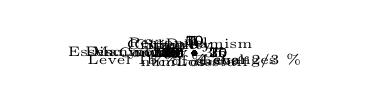
\begin{tikzpicture}[scale=1]
  \path (0:0cm) coordinate (O); % define coordinate for origin

  % draw the spiderweb
  \foreach \X in {1,...,\D}{
    \draw (\X*\A:0) -- (\X*\A:\R);
  }

  \foreach \Y in {0,...,\U}{
    \foreach \X in {1,...,\D}{
      \path (\X*\A:\Y*\R/\U) coordinate (D\X-\Y);
      \fill (D\X-\Y) circle (1pt);
    }
    \draw [opacity=0.3] (0:\Y*\R/\U) \foreach \X in {1,...,\D}{
        -- (\X*\A:\Y*\R/\U)
    } -- cycle;
  }

  % define labels for each dimension axis (names config option)
  \path (1*\A:\L) node (L1) {\parbox{3cm}{\centering \tiny Personnel \newline Level 1b \% -- Level 2/3 \%}};
  \path (2*\A:\L) node (L2) {\parbox{3cm}{\centering \tiny Criticality \newline Loss}};
  \path (3*\A:\L) node (L3) {\parbox{3cm}{\centering \tiny Size \newline num. of staff}};
  \path (4*\A:\L) node (L4) {\parbox{3cm}{\centering \tiny Culture \newline \% of chaos}};
  \path (5*\A:\L) node (L5) {\hspace{10mm}\parbox{3cm}{\centering \tiny Dynamism \newline \% changes}};

  %Units
  %Personel
  \draw (D1-1) node {\tiny 0 \hspace{2mm} 35};
  \draw (D1-2) node {\tiny 10 \hspace{2mm} 30};
  \draw (D1-3) node {\tiny 20 \hspace{2mm} 25};
  \draw (D1-4) node {\tiny 30 \hspace{2mm} 20};
  \draw (D1-5) node {\tiny 40 \hspace{2mm} 15};

  %Criticality
  \draw (D2-1) node {\hspace{-11mm} \tiny Comfort \hspace{2mm}};
  \draw (D2-2) node {\hspace{-15mm} \tiny Disc. money \hspace{2mm}};
  \draw (D2-3) node {\hspace{-18mm} \tiny Essen. money \hspace{2mm}};
  \draw (D2-4) node {\hspace{-7mm} \tiny Life \hspace{2mm}};
  \draw (D2-5) node {\hspace{-15mm} \tiny Many lives \hspace{2mm}};

  %Size
  \draw (D3-1) node {\hspace{-5mm}\tiny 5};
  \draw (D3-2) node {\hspace{-6mm}\tiny 10};
  \draw (D3-3) node {\hspace{-6mm}\tiny 30};
  \draw (D3-4) node {\hspace{-7mm}\tiny 100};
  \draw (D3-5) node {\hspace{-7mm}\tiny 300};

  %Culture
  \draw (D4-1) node {\hspace{-5mm}\tiny 90 };
  \draw (D4-2) node {\hspace{-5mm}\tiny 70 };
  \draw (D4-3) node {\hspace{-5mm}\tiny 50 };
  \draw (D4-4) node {\hspace{-5mm}\tiny 30 };
  \draw (D4-5) node {\hspace{-5mm}\tiny 10 };

  %Dynamism
  \draw (D5-1) node {\raisebox{3mm}{\tiny 50}};
  \draw (D5-2) node {\raisebox{3mm}{\tiny 30}};
  \draw (D5-3) node {\raisebox{3mm}{\tiny 10}};
  \draw (D5-4) node {\raisebox{3mm}{\tiny 5}};
  \draw (D5-5) node {\raisebox{3mm}{\tiny 1}};

  \draw [color=blue,line width=1.5pt,opacity=0.5]
    (D1-3) --
    (D2-1) --
    (3*\A:2.2*\R/\U) --
    (D4-2) --
    (D5-2) -- cycle;


\end{tikzpicture}
\caption{Radar chart showing deciding factors of the development method of our project}
\label{fig:developmentFactors}
\end{figure}

A polar chart showing the factors for our project is seen in Figure~\ref{fig:developmentFactors}.
As seen, must of the points are closer to the center than the periphery, this indicates that an agile method is preferred over a traditional one.

The personnel score is positioned in the middle because we consider ourselves above level 1b, but none or very few of us qualify as level 2 or three.


We will use a development approach similar to Scrum of Scrums.
The reason for this is three fold.
First of all we have a diverse target group (point \ref{enum:targetGroup}), that may make a big up front analysis and design difficult.
This leads us to choose an agile method due to ``I know it when I see it'' (IKIWISI), that is the customer does not know what she wants before she sees it.
This is also supported by the polar chart showing the development factors in Figure~\ref{fig:developmentFactors}

Secondly we are 14 group members divided into four groups (as point \ref{enum:groupSize} states) which is not handled very well in other agile methods such as XP, which dictates that all the developers should be in the same room. 
This is not the case for us as point \ref{enum:room} states.

The third reason is that we have a hard deadline (point \ref{enum:deadline}), which means that we have to hand in our project at a specific date.
Scrum of Scrums suggests that iterations (sprints) are time-boxed, which is ideal for us since we can cut less important features instead of missing the deadline.
This is also supported by point \ref{enum:passed}, because the end product is a working release although some features may have been cut.
The features cut may then be suggested to the group which is to take up this project next year.


\subsubsection{Refining SCRUM}
As point \ref{enum:manager} and \ref{enum:onsite} states, we have neither a project manager nor an available on-site customer.
We will handle the missing on-site customer by having shorter iterations and contacting the customers whenever an iteration is over.
Scrum of Scrums dictates that there should be a Scrum master in each subgroup.
Since none of us has used Scrum before, none of us are qualified to be Scrum master.
We are in an educational situation (see point \ref{enum:education}) so we will strive to allow every member to try to be Scrum master for a shorter time period.
This may not be ideal, but we consider it to be more important that every member of the subgroups tries to have the responsibility of a Scrum master than having only one member trying it and learning it well.

%\fixme{Kim: syntes at det skal skrives mere, her er nogle ideer (se comment)}
\begin{comment}
There is more:
*Scrum board
*The phases / meetings
**estimation
**sprint planning
*Scrum meetings
*Scrum of scrum def
*project manager progblem
\end{comment}


\subsection{Tools}
A series of tools are used in creation of this project.
These tools are briefly described in this section.
The tools that needs to be chosen must indeed complete some task, the tasks that needs a tool are: Version control, bug tracking, code documentation, and testing.

\subsubsection{Version Control}
All of us have been using subversion (SVN) in previous projects as the version controlling system.
SVN is a centralized solution \cite{subversion} with a single repository that the group members can update from and commit changes to.
This project does, however, differ from previous project with respect to the organization of groups; we are not one group of $x$ individuals, but rather one group consisting of some smaller subgroups, again consisting of individual persons.
This has lead us to choose a distributed solution rather than a centralized one.

The solutions considered are the distributed systems Git and Mercurial (Hg).
These systems are quite similar and the essential difference is that Hg is simpler than Git and Git is more flexible than Hg \cite{gitVsHg}.
A few of us have been using Hg and none of us have used Git, which leads us to choose Hg, such that we a little knowledge of the chosen system.

\subsubsection{Bug Tracking}
We need to have some way of communicating and tracking the defects or ``bugs'' that we will run into during our project.
The must important requirement for the tool we will use is that it should be able to track the bugs and make them easily available to the team that will continue on this project next year.
The tools that we are considering to use for bug tracking are Bugzilla \cite{bugzillaFeat} and Eventum \cite{eventumFeat}.
These tools are very similar in their sets of features.
When a bug is discovered a bug report must be added in the tool.
In the tools the members of a team can see the bugs and their status, and mark them as fixed when they are handled.

Since we have used Bugzilla as part of the course Test and Verification, it will save us the overhead of having to learn a new tool by select that over Eventum.
Furthermore, development of Eventum seem to be discontinued since the start of 2009 \cite{eventumDiscont}, which means that any defects that may be in the system are very unlikely to be fixed.
In conclusion we choose to use Bugzilla to track our bugs.

\subsubsection{Code Documentation}
%We want our documentation of our code to be as close to the code as possible.
%In particular we do not want to go back and forth between the source code and some other program when we are writing new functionality and documenting it.
We do not wish to use a tool that requires us to type in documentation externally from the code.
Therefore we want to use a tool like PHPDocumentor \cite{phpdocumentor} or PHPXref \cite{phpxref} to handle our documentation, since both of these reads comments in the source code and use it as documentation.
This gives us the ability to write code and documentation in the same file.
The syntax that both of these tools use is the same, which means that as long as we adhere to this syntax we can use either tool to generate documentation.

The difference between the two tools is that PHPDocumentor focus on giving a more diverse set of final documents (different HTML and PDF templates), where PHPXref focus more on the reference between classes, function, etc.
We use both tools such that we and the group that is to take up this project next year can choose the documentation they prefer.


\subsubsection{Testing}
The test tool that we want to use should be easily adapted by us, which leads us to look at tools using PHP, since that is the language we will be using to develop this project.
We also want the tests to survive after our work on the project ends, in particular the groups that is to take up this project next year should be able to use our test cases again.
We will be using the build in testing framework of Moodle \cite{moodletest}, which is based on SimpleTest \cite{simpletest}.
This should ensure that the test cases can be used next year as well and perhaps be part of the final product, should it ever be realeased to the public.














